\chapter{土地利用与土地覆盖变化模拟}\label{土地利用与土地覆盖变化模拟}
%\addcontentsline{toc}{chapter}{土地利用与土地覆盖变化模拟}

\section{模拟方案概述}
土地利用与土地覆盖变化是陆面模拟中重要强迫项之一,对模拟结果具有不可忽视的影响,特别是在局地及区域尺度。
目前CoLM模式对土地利用与土地覆盖变化的模拟可以分为三种方式:
\begin{enumerate}
    \item 通过人为设定不同年份的地表输入数据,此为静态方案;
    \item 逐年更新,采用同次网格类型(包括IGBP、PFT、PC和Urban)状态变量进行赋值(hot-start),新增加类型进行初始化(cold-start),为同类赋值方案(Same Type Assignment, SAT);
    \item 在方案2的基础上,利用地表覆盖转移矩阵,对状态变量赋值时保持物质和能量守恒,即守恒方案(Mass
and Energy Conservation, MEC)。
\end{enumerate}

静态方案通过\texttt{namelist DEF\_LC\_YEAR}指定地表覆盖数据年份。目前提供2001-2022年地表输入数据(采用MODIS地表覆盖数据为基础制作而成),运行时指定模式地表数据年份即可,通过以上设置生成地表数据,进行初始化及主程序编译,生成的程序会读入指定年份的地表数据。该方式设置简单,适用于不同年份地表数据气候态结果分析和地表覆盖变化影响机理研究。

同类赋值和守恒方案则通过\texttt{namelist DEF\_LULCC\_SCHEME}进行设置,当
\texttt{DEF\_LULCC\allowbreak \_SCHEME = 1}时为同类赋值方案,\texttt{DEF\_LULCC\_SCHEME = 2}时为守恒方案。

对于同类赋值和守恒方案,有几点需要说明:

1) 对于所模拟的年份,需要提前制作好地表数据,可通过类似静态方案设置\texttt{namelist DEF\_LC\_YEAR}逐年生成(由于生成地表数据需要大量计算资源,在目前阶段暂不采用代码自动实现的方式来生成LULCC地表数据,而是根据用户需求手动设置生成);

2) 对于为模式发展自行新增的状态变量并不能自动实现LULCC,需要手动添加对应的变量代码;

3) LULCC目前暂不支持USGS地表分类、生物地球化学模块及单点运行;

4) LULCC方案打开后LAI将会根据模式运行时间自动更新,覆盖\texttt{namelist DEF\- \_LAI\_CHANGE\_YEARLY}设置。


\section{LULCC运行基本流程}

{
\begin{figure}[htbp]
\centering
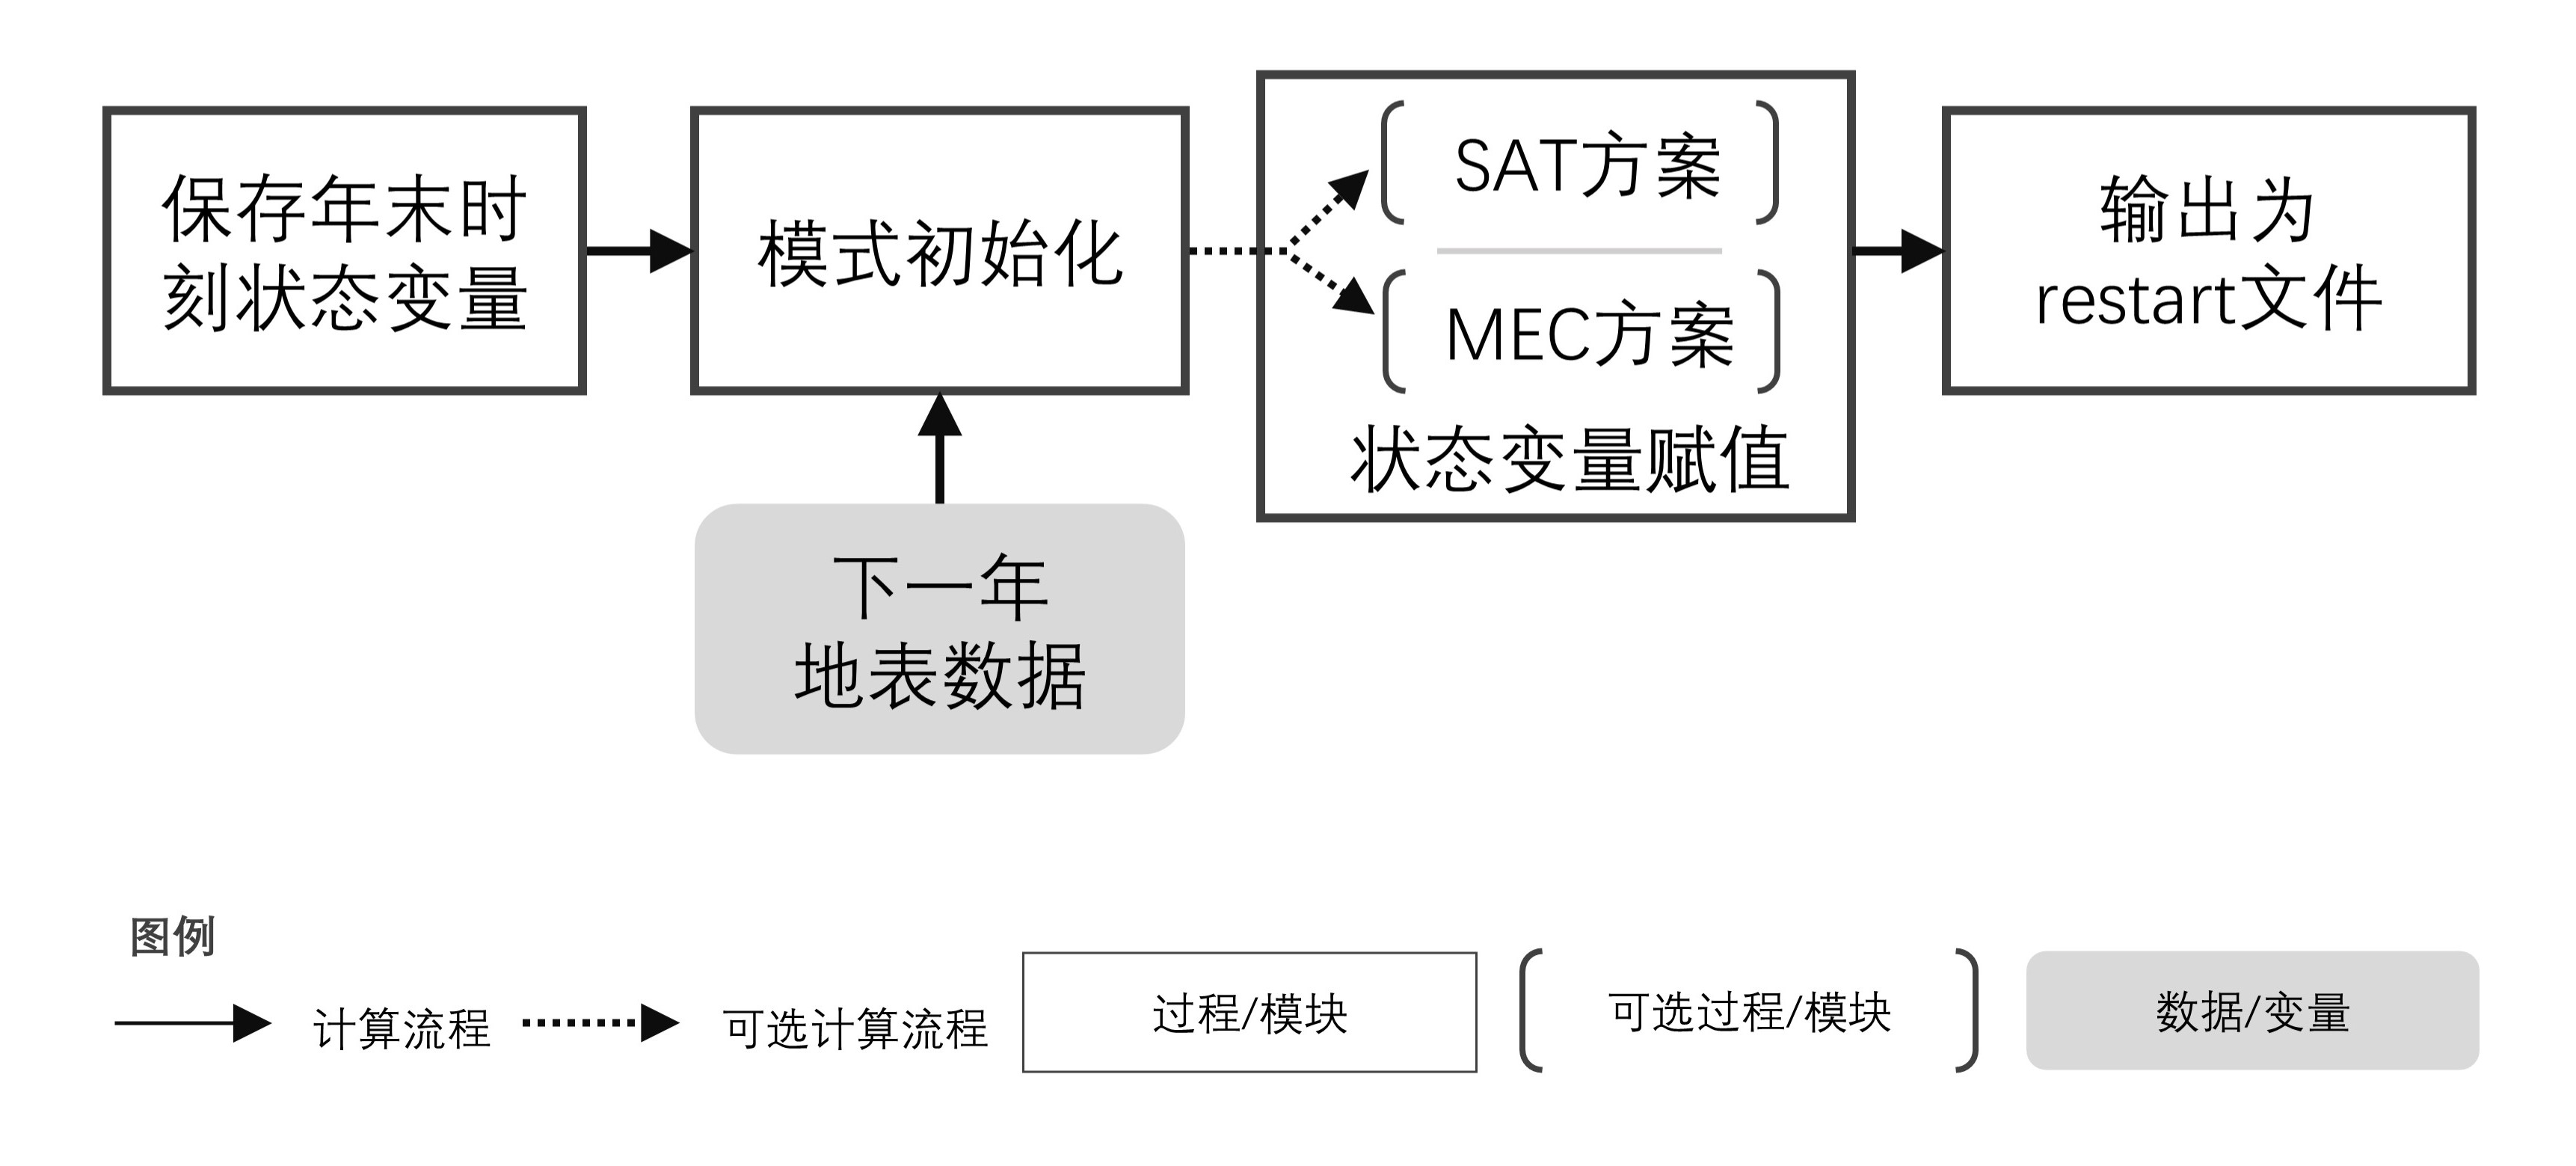
\includegraphics[width=0.85\columnwidth]{Figures/土地利用与土地覆盖变化模拟/LULCCDRIVER流程图.jpg}
\caption{LULCC主程序流程图 (MOD\_LULCC\_Driver.F90)}
\label{fig:LULCC主程序流程图}
\end{figure}
}

对于同类赋值方案和守恒方案,目前模式提供2001-2022年地表输入数据,运行时指定模式初始运行年份地表覆盖数据,并在\texttt{define.h}文件中打开土地利用与土地覆盖变化宏(\texttt{\#define LULCC}),即可每年动态更新地表数据。通过以上设置产生多年地表数据,使用开始年地表数据完成模式初始化(restart run方式除外),主程序会相应读入模型运行年份的地表数据。地表数据的更新在每年最后一个时间步长结束后进行。

状态变量也需随地表数据的更新而更新,具体过程如下:

\begin{enumerate}
\item 当运行到每年的最后一个时刻,首先将模式运行相关变量内存释放,以确保patch数目在模式的后续运行中能与新一年的地表数据匹配。

\item 然后执行LULCC主程序,即对restart run所需的相关变量进行调整,主要包含以下步骤:1. 首先将最后一个时刻的状态变量和常量保存,用于后续对新一年状态变量的赋值或调整;2. 根据新一年的地表数据运行\texttt{mkinidata},对新一年的变量进行初始化。若变量在后续没有进行赋值或调整,则会保持该初始化的值,如叶面积指数(LAI);3. 根据\texttt{DEF\_LULCC\_SCHEME}选项设置的LULCC方案进行变量调整。

\item 最后将调整完的所有变量重新输出到restart文件,作为新一年模式运行的初始值,并根据新一年的patch重新初始化大气强迫与通量数据。
\end{enumerate}

如图~\ref{fig:LULCC主程序流程图}所示,同类赋值与守恒方案的不同仅在于对状态变量的调整,地表数据的更新方式以及调整前的准备步骤是完全相同的。

\section{同类赋值方案-SAT}

对于同类赋值方案,这里的同类包括植被次网格类型LCT、PFT和PC,同时也适用于打开城市模式后城市分类。下一年初始的状态变量由上一年最后一个时刻相同次网格类型上保存的状态变量赋值,若下一年存在新增类型,则其状态变量由初始化的数值代替。

该方式实现容易,简单考虑地表数据逐年替换,后续需要新增变量也可很快加入。同类赋值方案比较适合一些快变过程变量模拟,比如反照率、温度模拟等。但对于一些慢变过程(具有较长时间记忆)变量,如土壤水等,建议采用下面守恒方案。

\section{守恒方案-MEC}

{
\begin{figure}[htbp]
\centering
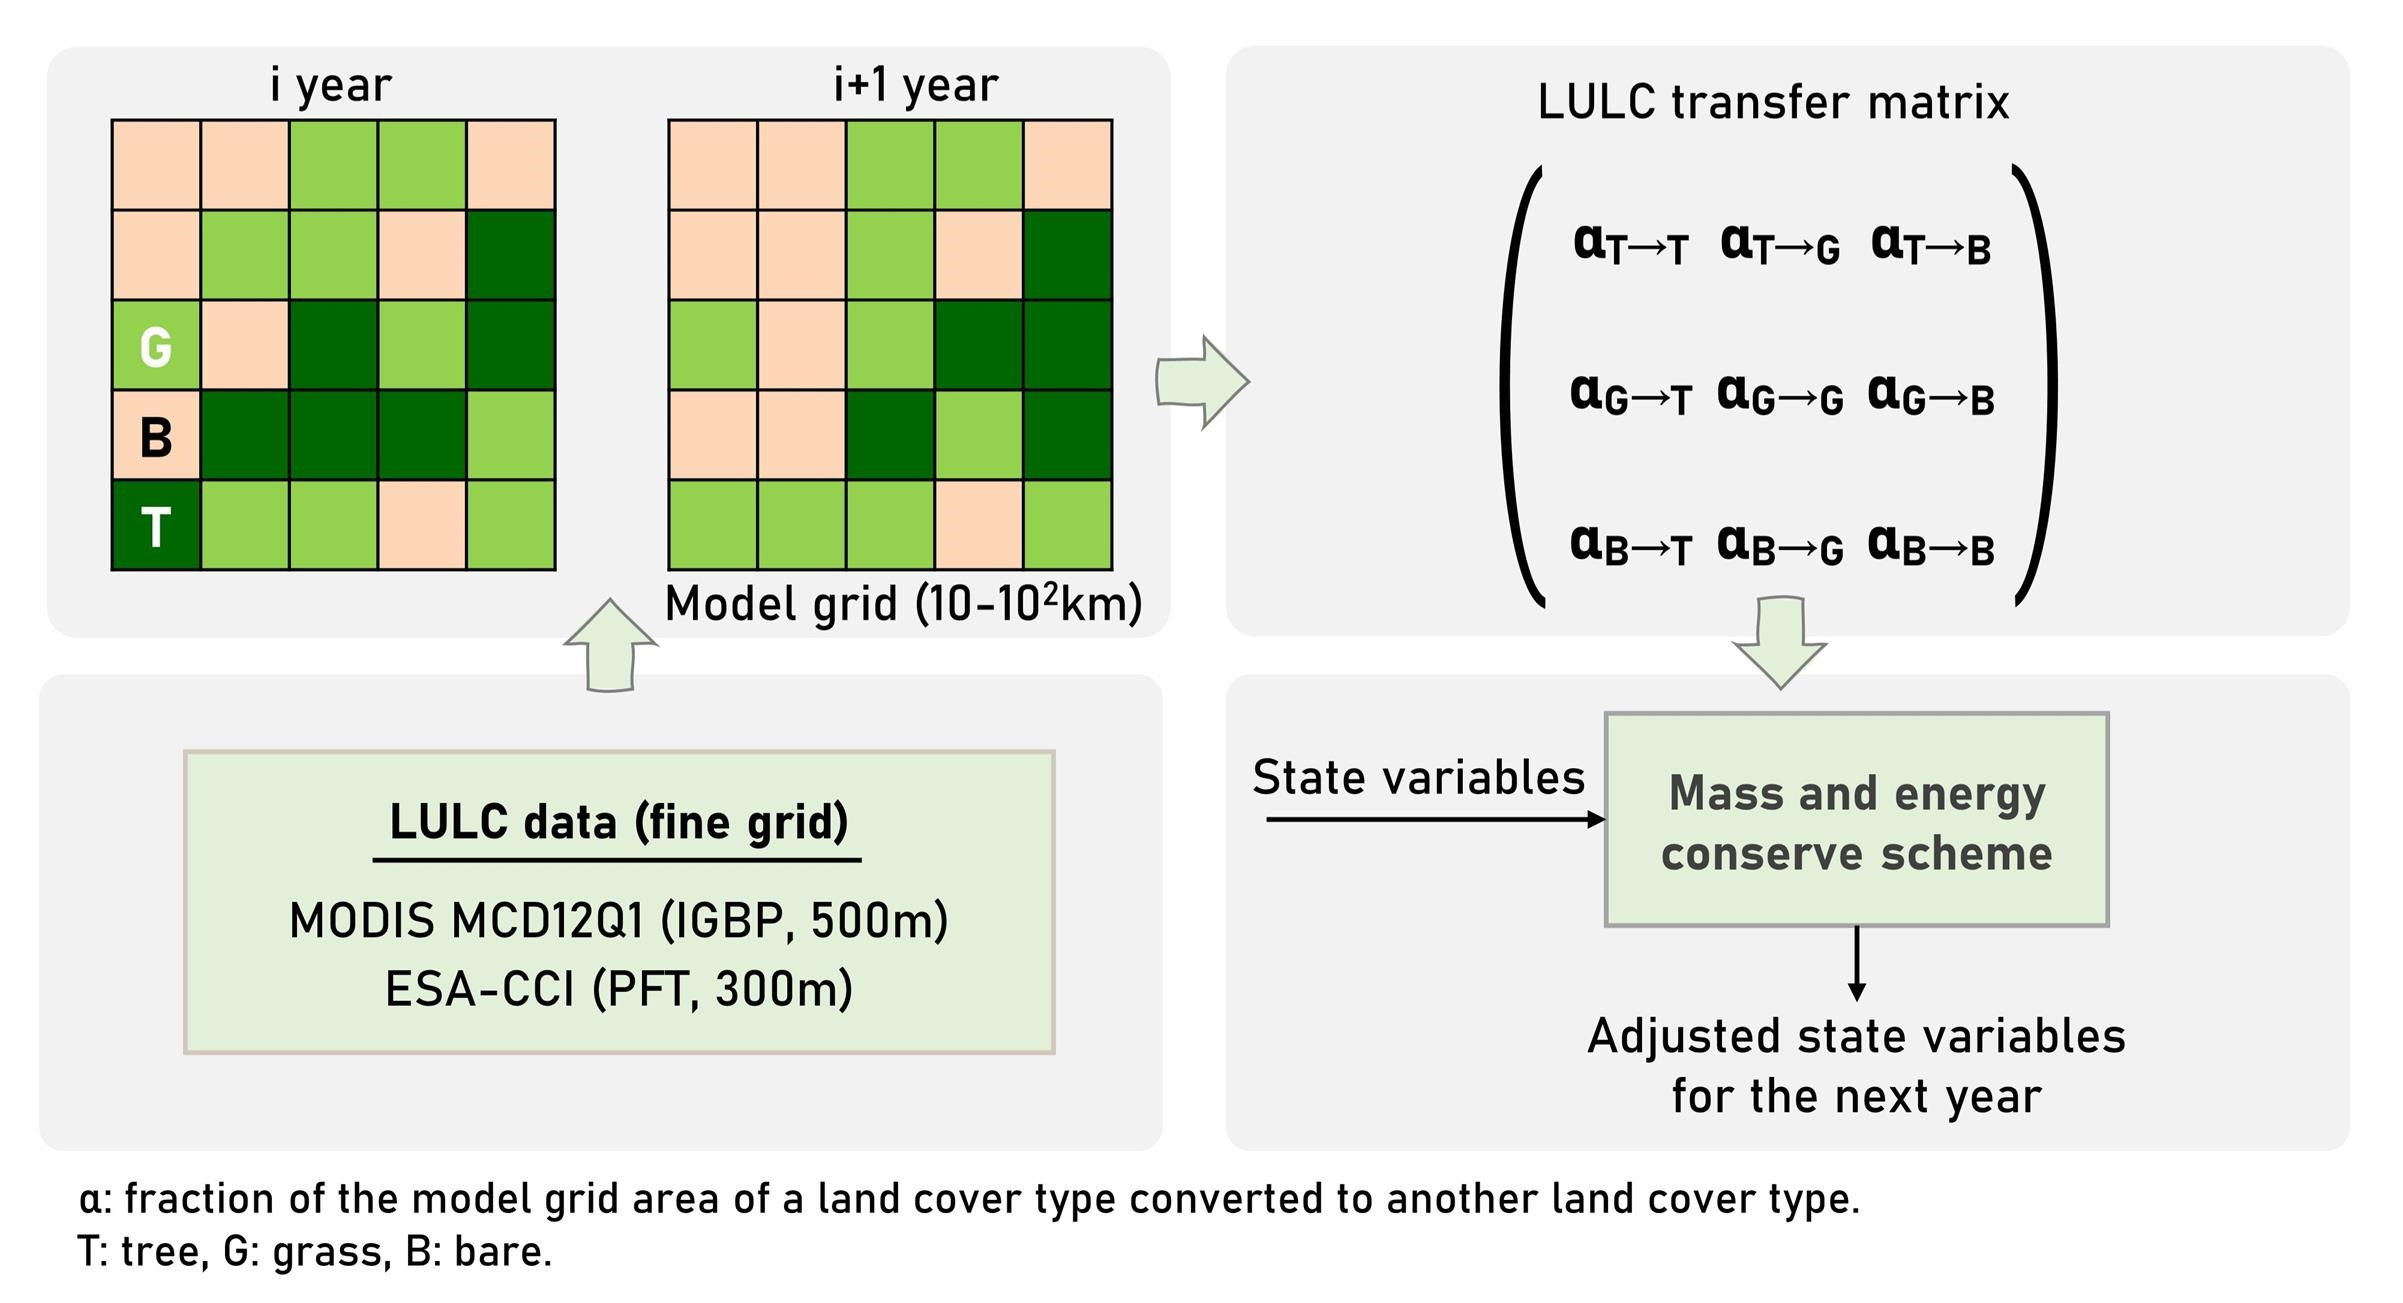
\includegraphics[width=1\columnwidth]{Figures/土地利用与土地覆盖变化模拟/LULCC流程图.png}
\caption{地表覆盖变化的物质能量守恒方案示意图}
\label{fig:LULCC流程图}
\end{figure}
}

在守恒方案中,变量的调整主要通过两个程序完成,即1) 制作相邻两年的地表覆盖追溯数据;2) 利用上一步生成的数据,对状态变量进行调整,以保持物质和能量守恒。

地表覆盖追溯转移矩阵的制作需首先在模式网格上获取今年的每一个patch所包含的pixel,以及pixel在去年的地表类型,对pixel的类型进行计数。然后计算每一种地表类型占网格面积(不考虑网格中的海洋面积)的比例,作为后续状态变量守恒调整的权重。该结果会作为诊断数据输出,可用于地表覆盖变化分析。

当获得每个patch的来源patch占比后,即可对restart文件中涉及变量的调整。守恒方案中的状态变量调整可以大致分为以下几种情况:


1) \textbf{物质守恒}。与物质相关的变量,如叶上的积水$L_{dew}$、土壤液态水含量$w_{liq}$、土壤固态水含量$w_{ice}$
、含水层水量$w_{a}$,新一年patch上的值采用来源patch的面积加权平均进行赋值。部分变量虽然不是守恒量,但也采用同样的方法进行调整,包括雪龄 (snow age) 、雪的有效粒径$snw\_rds$等。

2) \textbf{能量守恒}。与能量相关的变量,包括雪层和土壤层的温度$T$,是基于所有来源patch变化到新的温度之后,热量的变化总和为0的假设来计算:
\begin{equation}
T^{n} = \sum_{i = 1}^{np}{\ \lbrack T_{i}^{n - 1}\text{~}\text{*}\text{~}\frac{C_{vi}^{n - 1}\text{~}\text{*}\text{~}S_{i}^{n - 1}}{\sum_{i = 1}^{np}{(C_{vi}^{n - 1}\text{~}\text{*}\text{~}S_{i}^{n - 1})}}\text{]~~}}
\end{equation}
其中\(T_{i}^{n - 1}\)是去年来源patch的土壤温度,\(T^{n}\)是今年的patch的土壤温度,\(S_{i}^{n - 1}\)是来源patch的面积百分比,\(C_{vi}^{n - 1}\)是土壤热容量(单位:\( \rm Jm^{-2}K^{-1}\),\(C_{vi}^{n - 1}\)的计算同土壤温度计算\texttt{MOD\_GroundTemperature.F90}中的方案。因此土壤温度调整的权重为来源patch的面积与土壤热容量的乘积。

3) \textbf{通过物理过程计算调整}。经过以上物质和能量守恒调整后,一些变量会因物理过程的计算受到影响,此时需要根据物理过程部分的代码进行调整,包括雪层的厚度$\delta z$、雪层的深度$z$、雪水当量$W_{sno}$、积雪厚度$z_{sno}$、被积雪覆盖的地表面积比例$f_{sno}$、斑块中的有效植被比例$f_{sig}$等等。这些变量的调整需要首先确定雪的层数,雪的层数被设置为来源patch中面积占比最多的patch的雪层数,即以主要来源patch为准。其中每一层的含水量、含冰量以及雪的密度可通过来源patch对应层的数值做面积加权平均调整。当出现其他patch的雪层数多于主要patch的层数的情况时,则将多出来的部分采用同样的方式加到最上层。此时即可根据含水量、含冰量和雪的密度来计算雪层的厚度,同时也可计算出雪层的深度$z$、雪水当量$W_{sno}$和积雪厚度$z_{sno}$。被积雪覆盖的地表面积比例$f_{sno}$和斑块中的有效植被比例$f_{sig}$通过调用雪盖比例子程序\texttt{snowfraction}进行计算,同时将茎面积指数$SAI$更新。地表温度$T_{g}$采用调整后的最上层的温度(没有雪则采用土壤第一层的温度)。地下水位$z_{wt}$采用来源patch中水位最低的patch进行赋值。

4) \textbf{保持初始化或采用同类赋值}。叶面积指数$LAI$、茎面积指数$SAI$是在新一年初始化时从地表数据读取得到的。反照率$\alpha$、辐射吸收($ssun$, $ssha$)、消光系数($extkb$, $extkd$)、叶片温度$T_{leaf}$、植被覆盖度$f_{veg}$等根据新一年的植被状态进行初始化。与湖泊地表类型相关的变量如湖泊冻结比例$T$、湖泊温度$T_{lake}$等变量采用同类赋值方法。

当打开城市模型,每个存在的城市类别都单独成为一个patch,城市patch的变量调整采用同类赋值方案。但假如去年不存在该类城市patch,则会用patch所在网格中的其他城市类型patch的相关变量进行赋值。若去年的网格中也不存在城市patch,则采用初始化的值。下垫面与透水面相关的变量采用其来源patch中的土壤类型patch进行赋值。为与城市中的水量分量组成及计算保持一致,土壤液态水含量$w_{liq}$、土壤固态水含量$w_{ice}$和雪水当量$W_{sno}$都参考城市模型物理过程部分的代码重新进行调整。

目前的守恒调整仅考虑向土壤、城市、湿地、湖泊类型patch的转换,还未考虑向冰川类型的转换,冰川patch的变量采用同类赋值调整。当定义地表次网格方案为LULC\_PFT或LULC\_PC时,patch索引的变量调整与IGBP完全一致。由于所有pft共享土壤,pft/pc索引的变量采用同类赋值(例如$T_{leaf}\_p$、$L_{dew}\_p$、$f_{sig}\_p$),而$SAI_p$的计算与LULC\_IGBP类似,除了初始化之外,还考虑当前雪的覆盖情况,通过调用雪盖比例计算子程序\texttt{snowfraction\_pftwrap}进行调整。在patch尺度上,植被patch上的对应变量则按pft/pc的百分比重新进行加权平均计算。

守恒方案较前两种物理上更为合理,具有同类赋值方案的特点,同时满足物质和能量守恒。

%\end{parbox}